\documentclass{article}


\usepackage{circuitikz} %Für die Schaltpläne
\usepackage[T1]{fontenc}
\usepackage[utf8]{inputenc}

\usepackage{fancyhdr}
\usepackage{lettrine}
\usepackage{hyperref}
\usepackage{subcaption}
\usepackage{tikz}
\usepackage{cite}
\usepackage{listings}
\usepackage[nottoc, numbib]{tocbibind}
\usepackage{../assets/scripts/tex/color-env}
\usepackage[ngerman]{babel}
%\usepackage{amsmath,amsfonts,stmaryrd,amssymb} % Math packages

\usepackage{enumerate} % Custom item numbers for enumerations

\usepackage[ruled]{algorithm2e} % Algorithms

\usepackage[]{mdframed} % Allows defining custom boxed/framed environments


\mdfdefinestyle{info}{%
	topline=false, bottomline=false,
	leftline=false, rightline=false,
	nobreak,
	singleextra={%
		\fill[black](P-|O)circle[radius=0.4em];
		\node at(P-|O){\color{white}\scriptsize\bf i};
		\draw[very thick](P-|O)++(0,-0.8em)--(O);%--(O-|P);
	}
}

% Define a custom environment for information
\newenvironment{info}[1][Info:]{ % Set the default title to "Info:"
	\medskip
	\begin{mdframed}[style=info]
		\noindent{\textbf{#1}}
}{
	\end{mdframed}
}


\mdfdefinestyle{warning}{
	topline=false, bottomline=false,
	leftline=false, rightline=false,
	nobreak,
	singleextra={%
		\draw(P-|O)++(-0.5em,0)node(tmp1){};
		\draw(P-|O)++(0.5em,0)node(tmp2){};
		\fill[black,rotate around={45:(P-|O)}](tmp1)rectangle(tmp2);
		\node at(P-|O){\color{white}\scriptsize\bf !};
		\draw[very thick](P-|O)++(0,-1em)--(O);%--(O-|P);
	}
}

% Define a custom environment for warning text
\newenvironment{warn}[1][Warning:]{ % Set the default warning to "Warning:"
	\medskip
	\begin{mdframed}[style=warning]
		\noindent{\textbf{#1}}
}{
	\end{mdframed}
}


\usetikzlibrary{shapes}
    \usetikzlibrary{arrows}
    \usetikzlibrary{arrows.meta,topaths}
    \usetikzlibrary{bending}
    \usetikzlibrary{calc}
\title{Elektrotechnik 1 Praktikum 1}


\usepackage[
  includehead,
  headheight = 17mm,
  footskip = \dimexpr\headsep+\ht\strutbox\relax,
  tmargin = 0mm,
  bmargin = \dimexpr17mm+2\ht\strutbox\relax,
]{geometry}

\usepackage{anyfontsize}

\usepackage{xcolor}

\definecolor{DarkGreenBlue}{HTML}{264653}
\definecolor{LightGreenBlue}{HTML}{2A9D8F}
\definecolor{LightOrange}{HTML}{E9C46A}
\definecolor{DarkOrange}{HTML}{F4A261}
\definecolor{RedOrange}{HTML}{E76F51}
\definecolor{BrightRed}{HTML}{D62828}
\definecolor{DeepBlue}{HTML}{003049}

\definecolor{codegreen}{rgb}{0,0.6,0}
\definecolor{codegray}{rgb}{0.5,0.5,0.5}
\definecolor{codepurple}{rgb}{0.58,0,0.82}
\definecolor{backcolour}{rgb}{0.95,0.95,0.92}

\lstdefinestyle{code}{
    backgroundcolor=\color{backcolour},   
    commentstyle=\color{codegreen},
    keywordstyle=\color{magenta},
    numberstyle=\tiny\color{codegray},
    stringstyle=\color{codepurple},
    basicstyle=\ttfamily\footnotesize,
    breakatwhitespace=false,         
    breaklines=true,                 
    captionpos=b,                    
    keepspaces=true,                 
    numbers=left,                    
    numbersep=5pt,                  
    showspaces=false,                
    showstringspaces=false,
    showtabs=false,                  
    tabsize=2
}

\lstset{style=code}


\pagestyle{fancy}
\fancyhead[L]{\leftmark}
\fancyhead[R]{}
\fancyfoot[L]{}
\fancyfoot[C]{\thepage}
\fancyfoot[R]{
\includegraphics[scale=0.2]{../assets/images/haw.jpg}}
\renewcommand\headrulewidth{0.5pt}


\begin{document}


\thispagestyle{empty}
\begin{tikzpicture}[overlay,remember picture]
  \thispagestyle{empty}
  \fill[black!2] (current page.south west) rectangle (current page.north east);

  \begin{scope}[transform canvas ={rotate around ={45:($(current page.north west)+(-.5,-6)$)}}]

    \shade[rounded corners=18pt, left color=DarkGreenBlue, right color=LightGreenBlue] ($(current page.north west)+(-.5,-6)$) rectangle ++(9,1.5);

  \end{scope}

  \begin{scope}[transform canvas ={rotate around ={45:($(current page.north west)+(.5,-10)$)}}]

    \shade[rounded corners=18pt, left color=LightOrange,right color=DarkOrange] ($(current page.north west)+(0.5,-10)$) rectangle ++(15,1.5);

  \end{scope}

  \begin{scope}[transform canvas ={rotate around ={45:($(current page.north west)+(0.5,-10)$)}}]

    \shade[rounded corners=8pt, right color=DarkOrange, left color=LightOrange] ($(current page.north west)+(1.5,-9.55)$) rectangle ++(7,.6);

  \end{scope}

  \begin{scope}[transform canvas ={rotate around ={45:($(current page.north)+(-1.5,-3)$)}}]

    \shade[rounded corners=12pt, left color=DeepBlue!80, right color=DeepBlue!60] ($(current page.north)+(-1.5,-3)$) rectangle ++(9,0.8);

  \end{scope}

  \begin{scope}[transform canvas ={rotate around ={45:($(current page.north)+(-3,-8)$)}}]

    \shade[rounded corners=28pt, left color=BrightRed, right color=BrightRed!80] ($(current page.north)+(-3,-8)$) rectangle ++(15,1.8);

  \end{scope}

  \begin{scope}[transform canvas ={rotate around ={45:($(current page.north west)+(4,-15.5)$)}}]

    \shade[rounded corners=25pt, left color=RedOrange, right color=DarkOrange] ($(current page.north west)+(4,-15.5)$) rectangle ++(30,1.8);

  \end{scope}

  \begin{scope}[transform canvas ={rotate around ={45:($(current page.north west)+(13,-10)$)}},]

    \shade[rounded corners=22pt, left color=DeepBlue,right color=DarkGreenBlue] ($(current page.north west)+(13,-10)$) rectangle ++(15,1.5);

  \end{scope}

  \begin{scope}[transform canvas ={rotate around ={45:($(current page.north west)+(18,-8)$)}},]

    \shade[rounded corners=8pt, left color=DarkOrange] ($(current page.north west)+(18,-8)$) rectangle ++(15,0.6);

  \end{scope}

  \begin{scope}[transform canvas ={rotate around ={45:($(current page.north west)+(19,-5.65)$)}},]

    \shade[rounded corners=12pt, left color=RedOrange] ($(current page.north west)+(19,-5.65)$) rectangle ++(15,0.8);

  \end{scope}

  \begin{scope}[transform canvas ={rotate around ={45:($(current page.north west)+(20,-9)$)}}]

    \shade[rounded corners=20pt, left color=BrightRed, right color=BrightRed!80] ($(current page.north west)+(20,-9)$) rectangle ++(14,1.2);

  \end{scope}

  \draw[ultra thick,gray] ($(current page.center)+(5,2)$) -- ++(0,-3cm) node[midway,left=0.25cm,text width=5cm,align=right,black!75]{{\fontsize{25}{30} \selectfont \bf MP 1\\[10pt] Praktikum 1}} node[midway,right=0.25cm,text width=6cm,align=left,orange]{{\fontsize{70}{86} \selectfont 2021}};

  \node at ($(current page.center)+(0,-4)$) {{\fontsize{40}{72} \selectfont Erste Schritte: TM4C1294NCPDT}};

  \node[text width=8cm,align=center] at ($(current page.center)+(0,-6.5)$) {{\fontsize{16}{20} \selectfont \textcolor{orange}{ \bf 3. November 2021}} \\[3pt] Florian Tietjen 2519584\\[3pt] Emily Antosch 2519935};

\end{tikzpicture}

\newpage


\tableofcontents

\listoffigures

\lstlistoflistings

\newpage

\section{Einführung in den TM4C1294NCPDT}

Im ersten Praktikum wollen wir uns mit dem Evaluation Board TM4C1294NCPDT vertraut machen,
mit dem wir uns auch in den nächsten Praktika beschäftigen wollen. Dabei richten wir
über den Projektbrowser und den Projekteigenschaften alle wichtigen Eigenschaften ein,
testen erste Konsolenausgaben und lassen LEDs in bestimmten Blinkmustern aufleuchten.


\section{Print to Console}

\begin{task}
UIn der ersten Aufgabe wollen wir die Ausgabe in der Konsole des Code Composer Studios
betrachten. 
\end{task}
  
Für das Bearbeiten dieser Aufgabe nutzen wir den folgenden Code:

\begin{lstlisting}[language=c, caption={printToConsole.c}, captionpos=b]
/*
Mikroprozessortechnik - Praktikum 1 Aufgabe 1
Print to Console
Autoren: Emily Antosch und Florian Tietjen
Beschreibung: Dieses Programm gibt eine geordnete Ausgabe eines Zaehlers, eines Namens und einer Matrikelnummer in der Konsole aus.
*/


#include "inc/tm4c1294ncpdt.h"
#include <stdio.h>
#include <stdint.h>

int main(void)
{
    int i, cnt; // Initalisierung der Varibalen

    cnt = 0; // cnt beginnt bei 0

    // Dauerschleife fuer den Zaehler
     while (1)
     {
         printf("%05d\n", cnt); // Ausgabe des Zaehlers
         printf("Name: Emily Antosch \n"); // Ausgabe des Namens
         printf("Matr.No: 2519935 \n"); // Ausgabe der Matrikelnummer
         cnt++; // Zaehler erhoehen um 1
         for (i = 0; i < 500000; i++) // Warteschleife
             ;
     }
}

  
\end{lstlisting}

Dabei schließen wir das Evaluation Board an und führen das Programm dann im Debugmodus aus.
Auf der Konsole erscheint eine schnell wachsende Liste von dem eingegebnen Namen, der Matrikelnummer und der steigenden Zählervariable cnt. 
\subsection{Kurzfazit}
Das zeigt uns zum Einen, wie wir die 
printf-Funktion in Code Composer Studio zu nutzen haben, um in größeren Programmen, Fehler finden zu können, zum Anderen haben wir das Setup des Boards richtig gemacht und das Kompilieren und Ausführen von Programmen funktioniert.


\newpage

\section{Blinking LED}


\begin{task}
  UIn der zweiten Aufgabe wollen wir üben, mit der Hardware auf dem Board zu arbeiten und bestimmte Register anzusprechen.
\end{task}

Dazu verwenden wir den folgenden Code:

\begin{lstlisting}[language=c, caption={Code für das Blinkmuster}, captionpos=b]
/*
Mikroprozessortechnik - Praktikum 1 Aufgabe 2
Blinking LED
Autoren: Emily Antosch und Florian Tietjen
Beschreibung: Dieses Programm greift auf die Ports N, F zu, um ein
Blinkmuster zu realisieren
*/


#include <stdint.h>
#include "inc/tm4c1294ncpdt.h"

int main(int argc, char const *argv[])
{
    int i = 0;                      // => Deklaration und Initalisierung der Warte-Variable i
    SYSCTL_RCGCGPIO_R = 0x00001020; // => Aktivieren der Ports N und F
    i++;                         // => Erhoehen der Variable i um 1, warten auf Clock
    GPIO_PORTN_DEN_R = 0x03;     // => Enablen der Pins 0 und 1
    GPIO_PORTN_DIR_R = 0x03;     // => Richtung der Pins N 0 und 1 auf Ausgang
    GPIO_PORTF_AHB_DEN_R = 0x11; // => Enablen der Pins 0 und 4
    GPIO_PORTF_AHB_DIR_R = 0x11; // => Richtung der Pins F 0 und 4 auf Ausgang
    // => Dauerschleife zum Ausfuehren des Blinkmusters
    while (1)
    {
        GPIO_PORTN_DATA_R = 0x02;    // => Setzen der LED 1 auf ON
        for (i = 0; i < 500000; i++) // => Warten
            ;
        GPIO_PORTN_DATA_R = 0x01;    // => Setzen der LED 2 auf ON
        for (i = 0; i < 500000; i++) // => Warten
            ;
        GPIO_PORTN_DATA_R = 0x00;     // => Reset beider Outputs auf OFF
        GPIO_PORTF_AHB_DATA_R = 0x10; // => Setzen der LED 3 auf ON
        for (i = 0; i < 500000; i++)  // => Warten
            ;
        GPIO_PORTF_AHB_DATA_R = 0x01; // => Setzen der LED 4 auf ON
        for (i = 0; i < 500000; i++)  // => Warten
            ;
        GPIO_PORTF_AHB_DATA_R = 0x00; // Reset beider Outputs auf OFF
    }
}


\end{lstlisting}

Dabei verwenden wir die beiden Register F und N, in welchen die Pins für die LEDs auf dem Board sind. Wir setzen alle Pins auf Ausgang und Enablen diese. Im Nachgang setzen wir die jeweiligen Pins im entsprechenden Blinkmuster auf OFF oder ON mit einer Warteschleife dazwischen.

\subsection{Ausgabe des Programms}

Wir erkennen einen durchgängigen Verlauf der LEDs, bei dem die LEDs der Reihe nach aufleuchten und dann wieder ausgehen, sodass immer nur eine
LED zur Zeit eingeschaltet ist. Es entsteht der Effekt eines "laufenden" Lichts, welches sich immer von links nach rechts bewegt.

\newpage

\begin{figure}
    \centering
    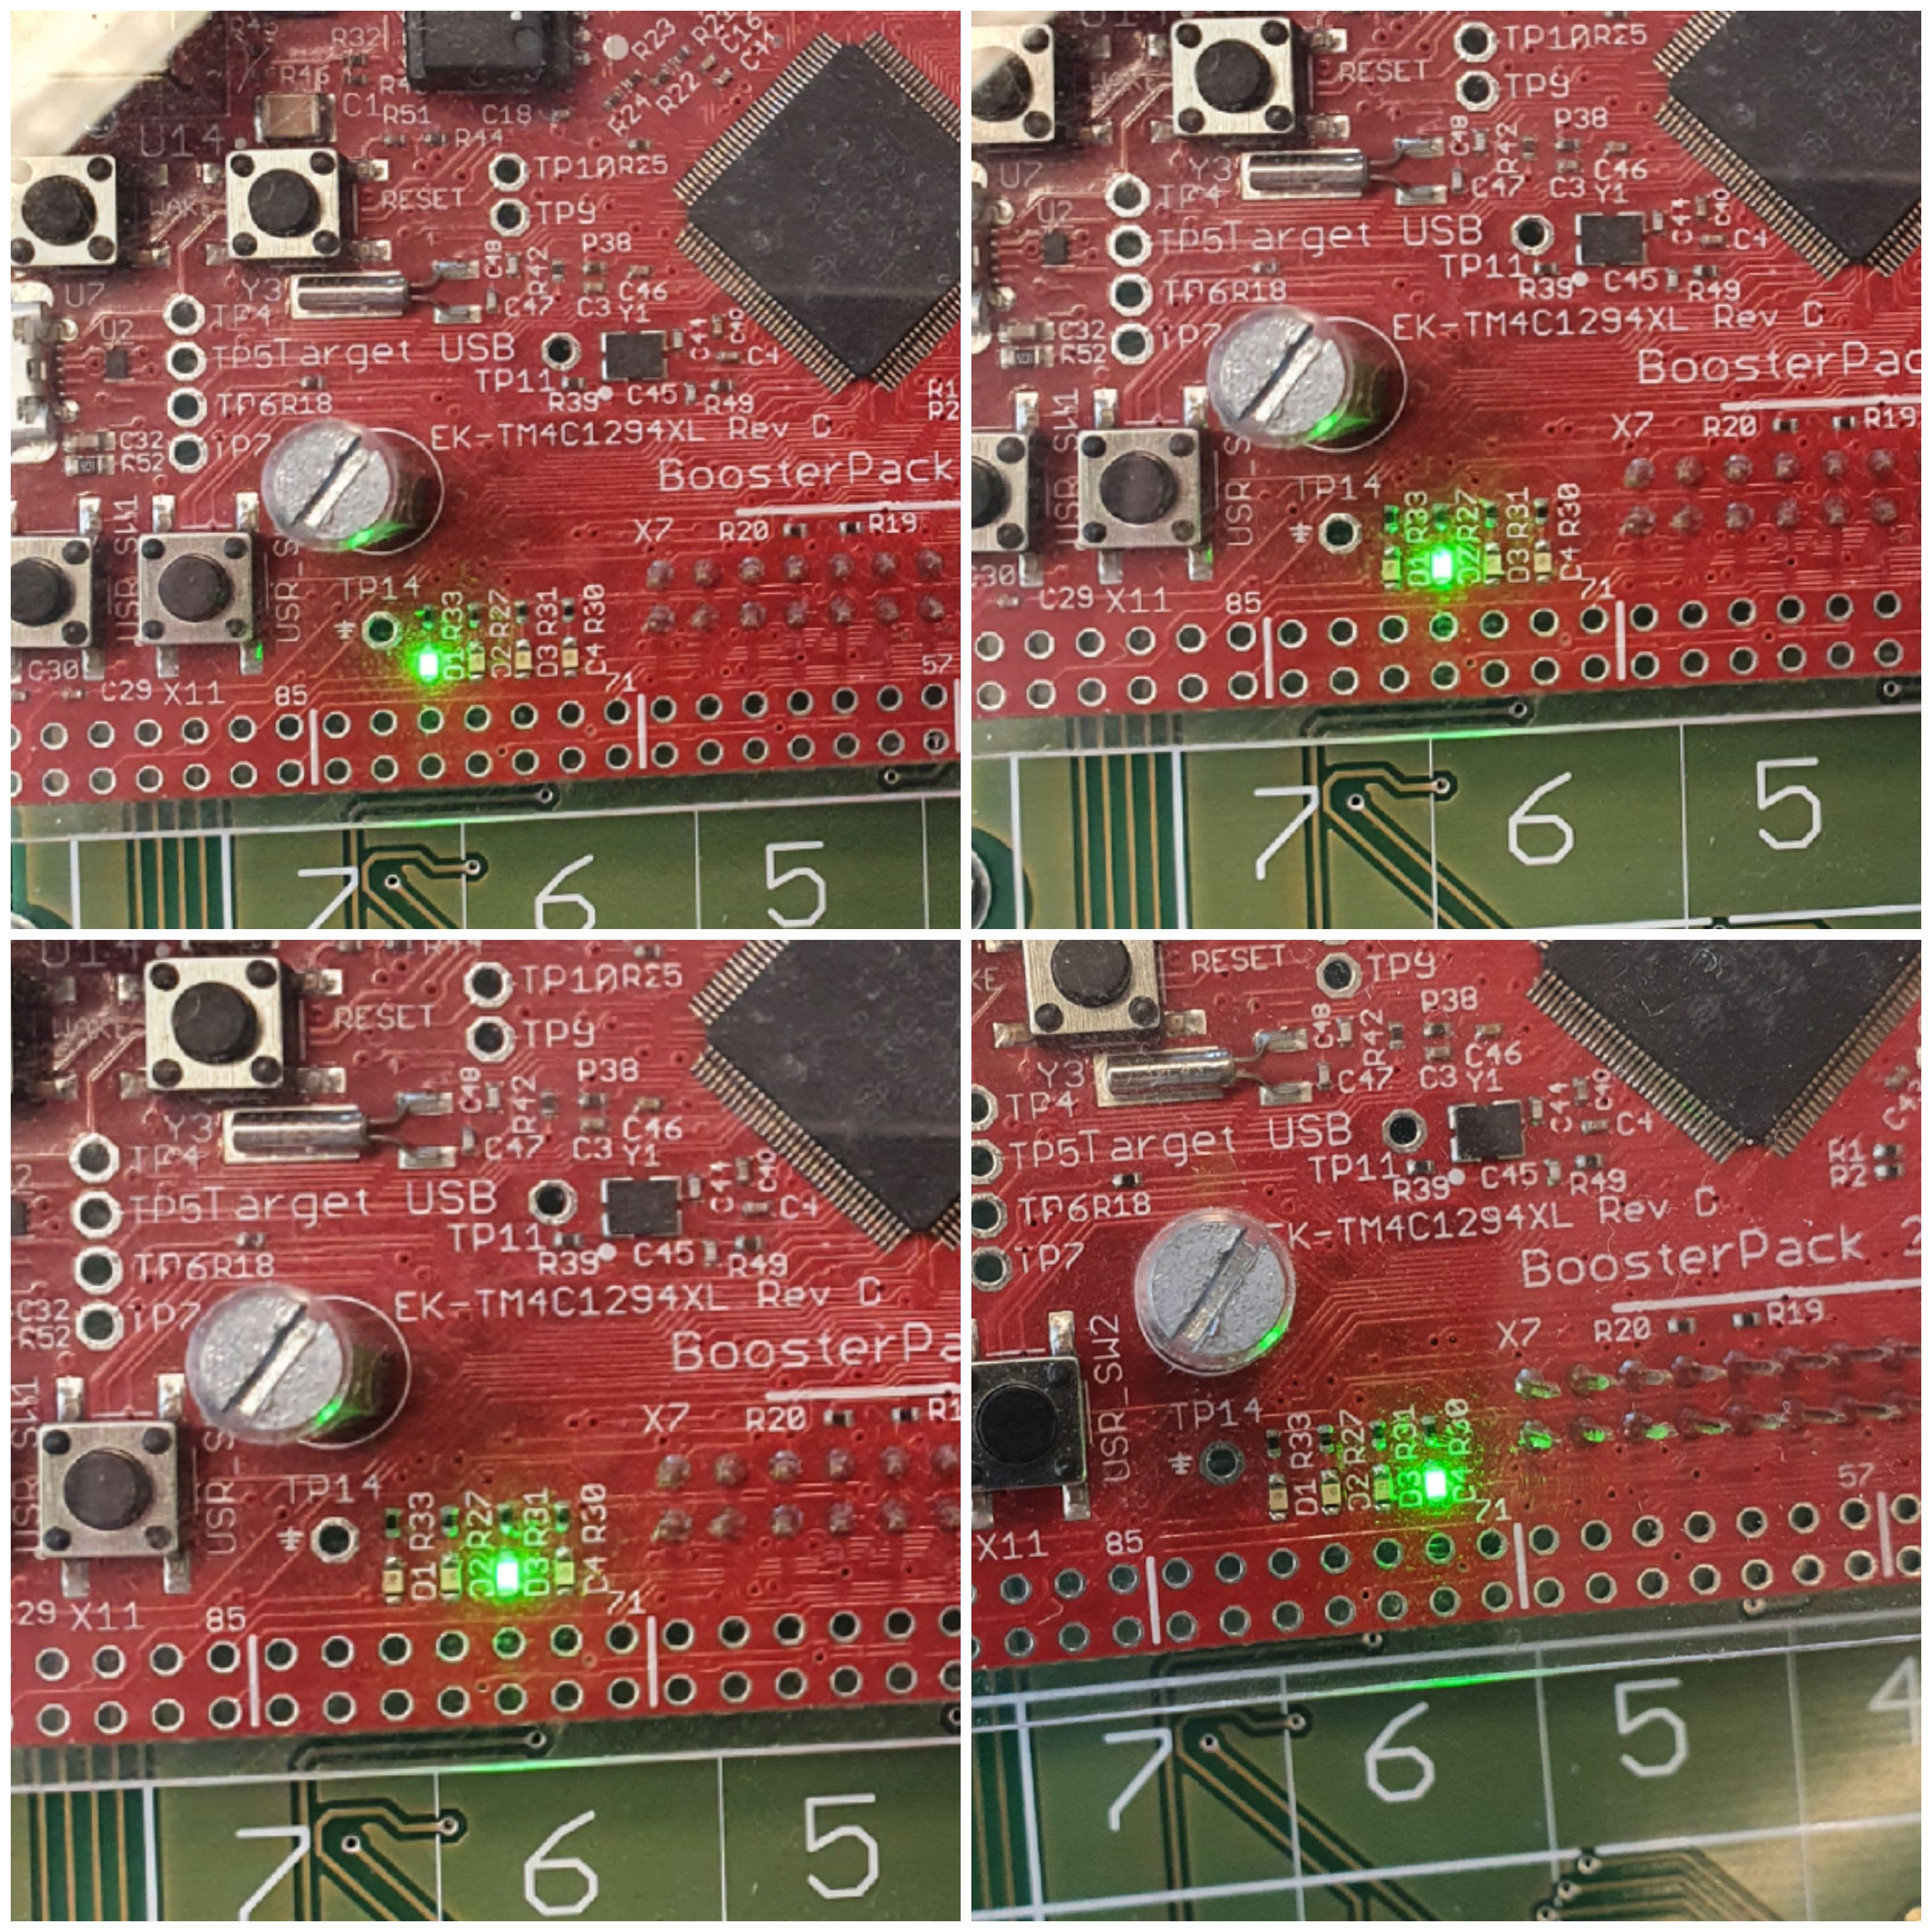
\includegraphics[width=\textwidth]{blinkLED.jpg}
    \caption{LED-Blinkmuster auf dem Evaluation Board}
    \label{fig:lbm}
\end{figure}


\subsection{Gleichzeitige Schaltung beider Eingänge in Port N}

Um beide LEDs an Port N gleichzeitig zu schalten müssen wir lediglich folgende Programmzeilen verwenden:
\begin{lstlisting}[language=c, caption={Port N Pins gleichzeitig schalten}, captionpos=b]
  GPIO_PORTN_DATA_R = 0x03;
  GPIO_PORTN_DATA_R = 0x00;
\end{lstlisting}
Dabei ist die erste Zeile das Schalten beider Pins auf ON, die zweite Zeile schaltet beide auf OFF. Dabei gilt $0x03_{16} = 0011_2$ und $0x00_{16} = 0000_2$, wobei eine $1$ auf einem bestimmten Port ein ON-Signal und eine $0$ ein OFF-Signal darstellt.

\subsection{Kurzfazit}

An dieser Aufgabe konnten wir erkennen, wie wir auf einfache Weise die Pins des Boards über die Ports ansprechen können. Für zukünftige Aufgaben haben wir die Chance, diese LEDs einzubauen.




\newpage

\section{Blinking LED mit Tasten}

\begin{task}
  UIm letzten Aufgabenblock wollen wir nun ein Blinkmuster mit dem integrieren einer %Tasterfunktion realisieren.
\end{task}

\begin{lstlisting}[language=c, caption={Code für das Blinkmuster mit Taster}, captionpos=b]
/*
Mikroprozessortechnik - Praktikum 1 Aufgabe 3
Blinking LED mit Taster
Autoren: Emily Antosch und Florian Tietjen
Beschreibung: Dieses Programm greift auf die Ports N, F und J zu, um ein
Blinkmuster mit Tastern zu realisieren
*/

#include <stdint.h>
#include <stdio.h>
#include "inc/tm4c1294ncpdt.h"

int main(int argc, char const *argv[])
{
    int i = 0;                      // => Deklaration und Initalisierung der Warte-Variable i
    unsigned char state;            // => Deklaration der State-Variable zum Abfragen des Schalterstandes
    SYSCTL_RCGCGPIO_R = 0x00001120; // => Aktivieren der Ports N, J und F
    while ((SYSCTL_PRGPIO_R & 0x00001120) == 0) // => Warten bis Clocksignal anliegt
        ;
    i++;                         // => Erhoehen von i um 1, warten auf Clock
    GPIO_PORTN_DEN_R = 0x03;     // => Enablen der Pins N 0 und 1
    GPIO_PORTN_DIR_R = 0x03;     // => Richtung der Pins N 0 und 1 auf Ausgang
    GPIO_PORTJ_AHB_DEN_R = 0x03; // => Enablen der Pins J 0 und 1
    GPIO_PORTJ_AHB_PUR_R = 0x03; // => Weak-Pull-Up aktivieren fuer die Pins J 0 und 1
    GPIO_PORTJ_AHB_DIR_R = 0x00; // => Richtung der Pins J 0 und 1 auf Eingang
    GPIO_PORTF_AHB_DEN_R = 0x11; // => Enablen der Pins F 0 und 4
    GPIO_PORTF_AHB_DIR_R = 0x11; // => Richtung der Pins F 0 und 4 auf Ausgang
    // => Dauerschleife zum Ausgeben der Blinkmuster
    while (1)
    {
        state = GPIO_PORTJ_AHB_DATA_R; // Abfragen des Schalterstandes

        if (state == 0x02) // Wenn Schalter 1 gedrueckt
        {
            GPIO_PORTN_DATA_R = 0x02;    // LED 1 leuchtet
            for (i = 0; i < 500000; i++) // Warten
                ;
            GPIO_PORTN_DATA_R = 0x01;    // LED 2 leuchtet
            for (i = 0; i < 500000; i++) // Warten
                ;

        }
        else if (state == 0x01) //Wenn Schalter 2 gedrueckt
        {
            GPIO_PORTF_AHB_DATA_R = 0x10; // LED 3 leuchtet
            for (i = 0; i < 500000; i++)  // Warten
                ;
            GPIO_PORTF_AHB_DATA_R = 0x01; // LED 4 leuchtet
            for (i = 0; i < 500000; i++)  // Warten
                ;

        }
        else if (state == 0x00) // Wenn beide Schalter gedrueckt
        {
            GPIO_PORTN_DATA_R = 0x02;     // LED 1 leuchtet
            GPIO_PORTF_AHB_DATA_R = 0x10; // LED 3 leuchtet
            for (i = 0; i < 500000; i++)  // Warten
                ;
            GPIO_PORTN_DATA_R = 0x01;     // LED 2 leuchtet
            GPIO_PORTF_AHB_DATA_R = 0x01; // LED 4 leuchtet
            for (i = 0; i < 500000; i++)  // Warten
                ;

        }
        GPIO_PORTN_DATA_R = 0x00;     // Reset der LEDs 1 und 2
        GPIO_PORTF_AHB_DATA_R = 0x00; // Reset der LEDs 3 und 4
    }
}

  
\end{lstlisting}

Der Programmcode lässt uns nun die folgenden Eigenschaften realisieren:
\begin{itemize}
  \item Beim Drücken des Taster 1 blinken die LEDs 1 und 2 abwechselnd
  \item Beim Drücken des Taster 2 blinken die LEDs 3 und 4 abwechselnd
  \item Beim Drücken beider Taster blinken jeweils LEDs 1 und 2 und LEDs 3 und 4 paarweise abwechselnd
\end{itemize}

\subsection{Weak-Pull-Up-Widerstand}
737ms
Wichtig für die korrekte Funktion der Taster ist ein Weak-Pull-Up-Widerstand. Dieser zieht im Fall, dass der Taster nicht gedrückt ist, den Pin auf ein ON-Signal. Ohne Pull-Up-Widerstand würde der Eingang bei nicht gedrücktem
Taster in der Luft hängen. Er wäre also weder klar definiert logisch $1$ oder $0$ und wäre zudem stark beeinflussbar von äußeren Einflüssen (Induktivitäten).
Ist der Taster jedoch gedrückt, so ist der PIN mit GND verbunden und ist in jedem Fall logisch $0$.
\newpage
\subsection{Oszilloskop: Messung der Taktfrequenz}

Um einen Einblick in die Verarbeitung der verwendeten Befehle zu bekommen, wollen wir nun uns einmal anschauen, mit welcher Periodendauer das paarweise abwechselnde Aufblicken der LED erfolgt.

\begin{figure}[h]
  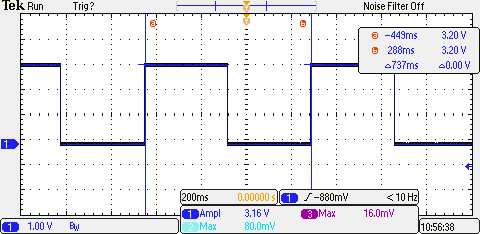
\includegraphics[width=\textwidth]{TEK00008.PNG}
  \caption{Verlauf der Spannung $U_F$ an einer der LEDs mit Verzögerung $i < 500000$} 
\end{figure}

Im oberen Beispiel haben wir den Verlauf der Spannung an einer LEDs beim Betätigen des entsprechenden Tasters aufgezeichnet. Die Verzögerung, die wir über die for-Schleife eingebaut haben, beträgt wie im Code-Beispiel $i < 500000$.

\begin{figure}[h]
  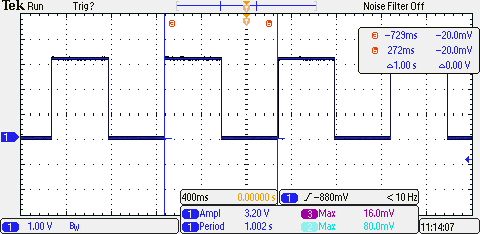
\includegraphics[width=\textwidth]{TEK00009.PNG}
  \caption{Verlauf der Spannung $U_F$ an einer der LEDs mit Verzögerung $i < 678426$}
\end{figure}

Im nächsten Beispiel haben wir die Verzögerung auf $\Delta t = 1s$ angepasst, indem wir $f_{1s} = \frac{f_{737ms}}{737ms} = \frac{500000}{737ms} \approx 678426 Hz$ gerechnet haben. Wir erkennen eine kleine Abweichung der Messung von $2ms$. 
\subsection{Kurzfazit}
Wir haben nun unser erstes eigenes Programm auf der Grundlage von der zweiten Aufgabe erstellen können. Auch den Umgang mit dem Oszilloskop konnte erneut geübt und vertieft werden, sodass wir für die nächsten Praktika besser vorbereitet sind. Diese kann aus sowohl Ungenauigkeiten der Messstrecken, sowie Fehler beim Ablesen der ursprünglichen Werte entstanden sein. 

\section{Konklusion}

Uns ist es gelungen, die Bedienung von CCS zu lernen und ein erstes Projekt richtig aufzusetzen. Die erste Arbeit mit Ports und Registern war erfolgreich und wir haben es geschafft, Zustände auf Ausgänge zu schreiben, sowie Taster als Eingangssignale einzulesen. Das erste eigene Programm haben wir ebenfalls zu Laufen bekommen und den erwünschten Effekt als Blinkmuster auf dem Board zu erhalten.

\end{document}